% \chapter{Overview}
This chapter provides an overview over different aspects that we need to take into consideration when developing a new design for MONDRIAN. These aspects will explain why we came up with certain design principles.

\subsection{Goals}
For our new design to comply with the original specification of MONDRIAN, we need to make sure that the logically centralized nature of MONDRIAN is preserved. Furthermore, we should at least logically still have just one \acs{TP} per site. Regarding the cryptographic operations a \acs{TP} performs, we still require a site-to-zone level granularity for the symmetric keys. Considering the format of the policies, we still want a mapping between the 5-tuplet to one of the three actions as described in formula \ref{policy}. Any of the five properties can be specified as a wildcard and the protocols we consider in the policies are the transport layer protocols \acs{TCP} and \acs{UDP}. Finally, we want the entire mechanism to be easily integratable into the existing infrastructure we typically find in a modern data center.

%\todo{\\
%    - Logically Centralized property must be preserved\\
%    - Concept of one TP per site should stay the same \\
%    - Encryption/authentication on site-to-zone level\\
%    - Integrateable in DCs\\
%    - nature of policies should be preserved (support for wildcards, 3 actions + default, proto=transport layer)
%}
\subsection{Assumptions}
In order to justify the design decisions we're making, we have to define what we assume about the data centers in which we want to employ MONDRIAN. Firstly, we assume that the data centers use \acs{SDN} and in particular have OpenFlow switches already in place. Then we assume that the different \acs{SDN} components are placed with great care into the Service Function Chain (\acs{SFC}), meaning that if MONDRIAN decides to disallow a zone transition, no other service function will allow the zone transition. We also require that the \acs{SDN} installation follows best practices, such that we can rely on OpenFlow to work as expected, without any attacker being able to interfere with the protocol.% and that OpenFlow traffic is secured using \acs{TLS} (\acl{TLS}), which unfortunately is not mandatory in OpenFlow \cite{agborubere2017openflow}. \todo{rewrite and if TLS stuff is removed make sure TLS is written out somewhere}

Regarding robustness and resiliency, we assume that standard mechanisms are in place to ensure fast failover and disaster recovery. Standard backup procedures should be applied to backup MONDRIAN specific data just as any other security relevant data.

Finally, we assume that there is an existing \acs{PKI} (\acl{PKI}) in place, which ensures the security of all traffic that is using asymmetric cryptography. The root certificate will be present wherever it is needed.
%\todo{\\
%    - Networking happens using SDN (OpenFlow Switches)\\
%    - Placement of SDN components in the service function chain happens with great care\\
%    - Security of SDN communication is ensured using best practices \cite{agborubere2017openflow}\\
%    - PKI is in place\\
%    - Standard mechanisms for resiliency are in place 
%}
\subsection{Requirements}
As discussed in section \ref{Data Center Networking}, it is essential that new components in a data center don't divert traffic from the original route, as it is most likely the optimal route for this specific application. Especially east-west traffic cannot be subject to any delays or diversions. This means that zone transitions need to be authorized wherever routing is performed since zone transitions are always transitions into other subnets, which requires a routing functionality to be in place. In \acs{SDN} based data center networks, routing can happen at any \acs{SDN} switch.

Finally, the solution must be scalable and integrate well with already existing technologies, first and foremost with \acs{SDN}.

%\todo{ \\
%    - Traffic should not be diverted -- transitions checked where routing happens \\
%    - East-west performacne can not be compromised \\
%    - Solution must be scalable and integrate well with existing technologies 
%}
\subsection{Design Principles}
Due to the end-host anonymity MONDRIAN provides, it is necessary to decrypt inter-domain traffic at the gateway of a data center. As soon as a packet enters the data center's network fabric, it needs to be known who the end-hosts are, such that routing can be performed. For this to happen, we need to lift end-host anonymity and hence decrypt the MONDRIAN packet. However, if we placed the \acs{TP} at the gateway of a data center, then all of the east-west traffic would be heavily diverted and congestion would be unavoidable. In order to prevent traffic from being diverted, we need to implement the functionality of the Transition Module as close to the end-hosts as possible. Meaning, it should be implemented in the virtual switches of the hypervisors. 

Since the functionality of the Authentication Module and the functionality of the Transition Module can't be implemented at the same physical location, we need to virtualize the concept of a \acs{TP} and introduce a virtual component we call \acs{vTP} (\acl{vTP}). A \acs{vTP} consists of an \textbf{Endpoint \acs{TP}}, implementing the functionality of the Transition Module by incorporating an \acs{SDN} approach and a \textbf{Gateway \acs{TP}}, implementing the functionality of the Authentication Module by following a classical \acs{VM} / container-based \acs{NFV} approach. 

Figure \ref{vTP Overview} shows the schematic setup of a \acs{vTP}. Even though there is just one Gateway \acs{TP} and one Endpoint \acs{TP} present in the figure, there's nothing preventing us from having multiple instances of these components to improve scalability and robustness. Note that for the setup to be a proper MONDRIAN deployment, we also need a MONDRIAN controller, which is connected to both the Gateway \acs{TP} and the Endpoint \acs{TP}. The end-hosts will be connected to the switches which are managed by the \acs{SDN} controller hosting the Endpoint \acs{TP} as a business application. The Gateway \acs{TP} will on the one side be connected to the outside world, namely the Internet or some \acs{WAN}, whereas on the other side it will be connected to a gateway, which is responsible for setting up the routes for the inter-domain traffic. It's important to note that neither the Endpoint \acs{TP} nor the Gateway \acs{TP} are responsible for routing activities.

%\todo{continue here... explain connectivity with mondiran controller, endpoint tp = sdn app, gateway tp = VM}

\begin{figure}[t]
	\centering
	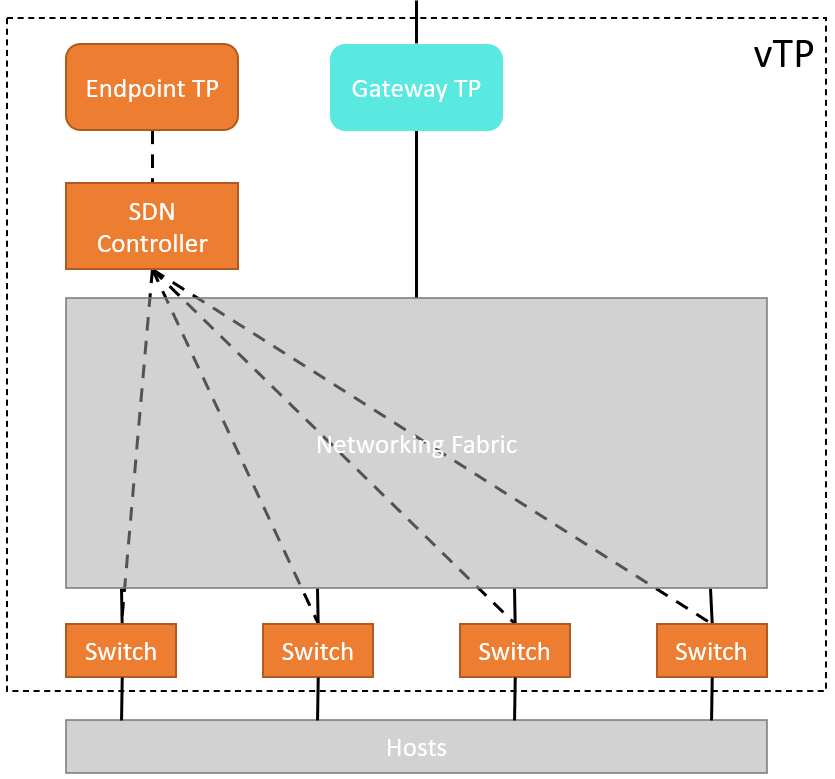
\includegraphics[width =0.48\textwidth]{img/vTP2.png}
	\caption{Conceptual overview of a \acl{vTP}}
	\label{vTP Overview}
\end{figure}

%\todo{ \\
%    - vTP keeps it logically centralized \\
%    - Splitting up the TP (explain why decryption needs to happen at the Gateway and why authorization needs to happen close to the Hosts) \\
%    - Discuss placement and connectivity of components [Fig]
%}